\section{Result}
\subsection{Simulation Studies}
The simulation is based on 806 ADNI participants having both NGS and MRI profiles. The 3D cortex were built from the MRI using Freesurfer~\cite{FS:Intro}. In each iteration we pick a gene $\bs{G}$ and a cortex region $\bs{V}$ of 512 vertices (roughly an oval with 28mm diameter), we then assign effect drawn from standard normal to 5\% of the genomic and imaging variants. From these variants we first generate two phenotypes solely based on genomic or imaging effect, $\bs{Y}_G$ and $\bs{Y}_V$, respectively, then add them up to get an additve effect $\bs{Y}_A$, then add their entry-wise product for an interactive effect $\bs{Y}_I$.
\begin{equation}\label{eq:SM1}
  \begin{split}
    \bs{Y}_G &= \bs{\beta}_G \bs{X}_G + \bs{\epsilon}_G, \quad \beta_{.G} \sim \bs{N}(0,1) \bs{Bernoulli}(0.05), \\
    \bs{Y}_V &= \bs{\beta}_V \bs{X}_V + \bs{\epsilon}_V, \quad \beta_{.V} \sim \bs{N}(0,1) \bs{Bernoulli}(0.05), \\
    \bs{Y}_A &= \bs{Y}_G + \bs{Y}_V, \qquad \bs{Y}_I = \bs{Y}_A + \bs{Y}_G \circ \bs{Y}_V.
  \end{split}
\end{equation}

\subsubsection{Performance of Joint Test}
We would like to see if the joint test overpower the genetic test when imaging is a contributor of the phenotype, either as a mediator (through interaction) or not. Also of interest is the performance of the joint test when the model is redundant, that is, applying the joint test while the phenotype is purely genomic or imaging based. The power of the joint statistic $U_J$ versus genomic based $U_V$ and imaging based $U_G$, under 8 sample sizes and 4 types of effects in (\ref{eq:SM1}), are shown in Figure~\ref{fig:PWR_CNT_KNL}.
\begin{figure}[!htbp]
  \centering
  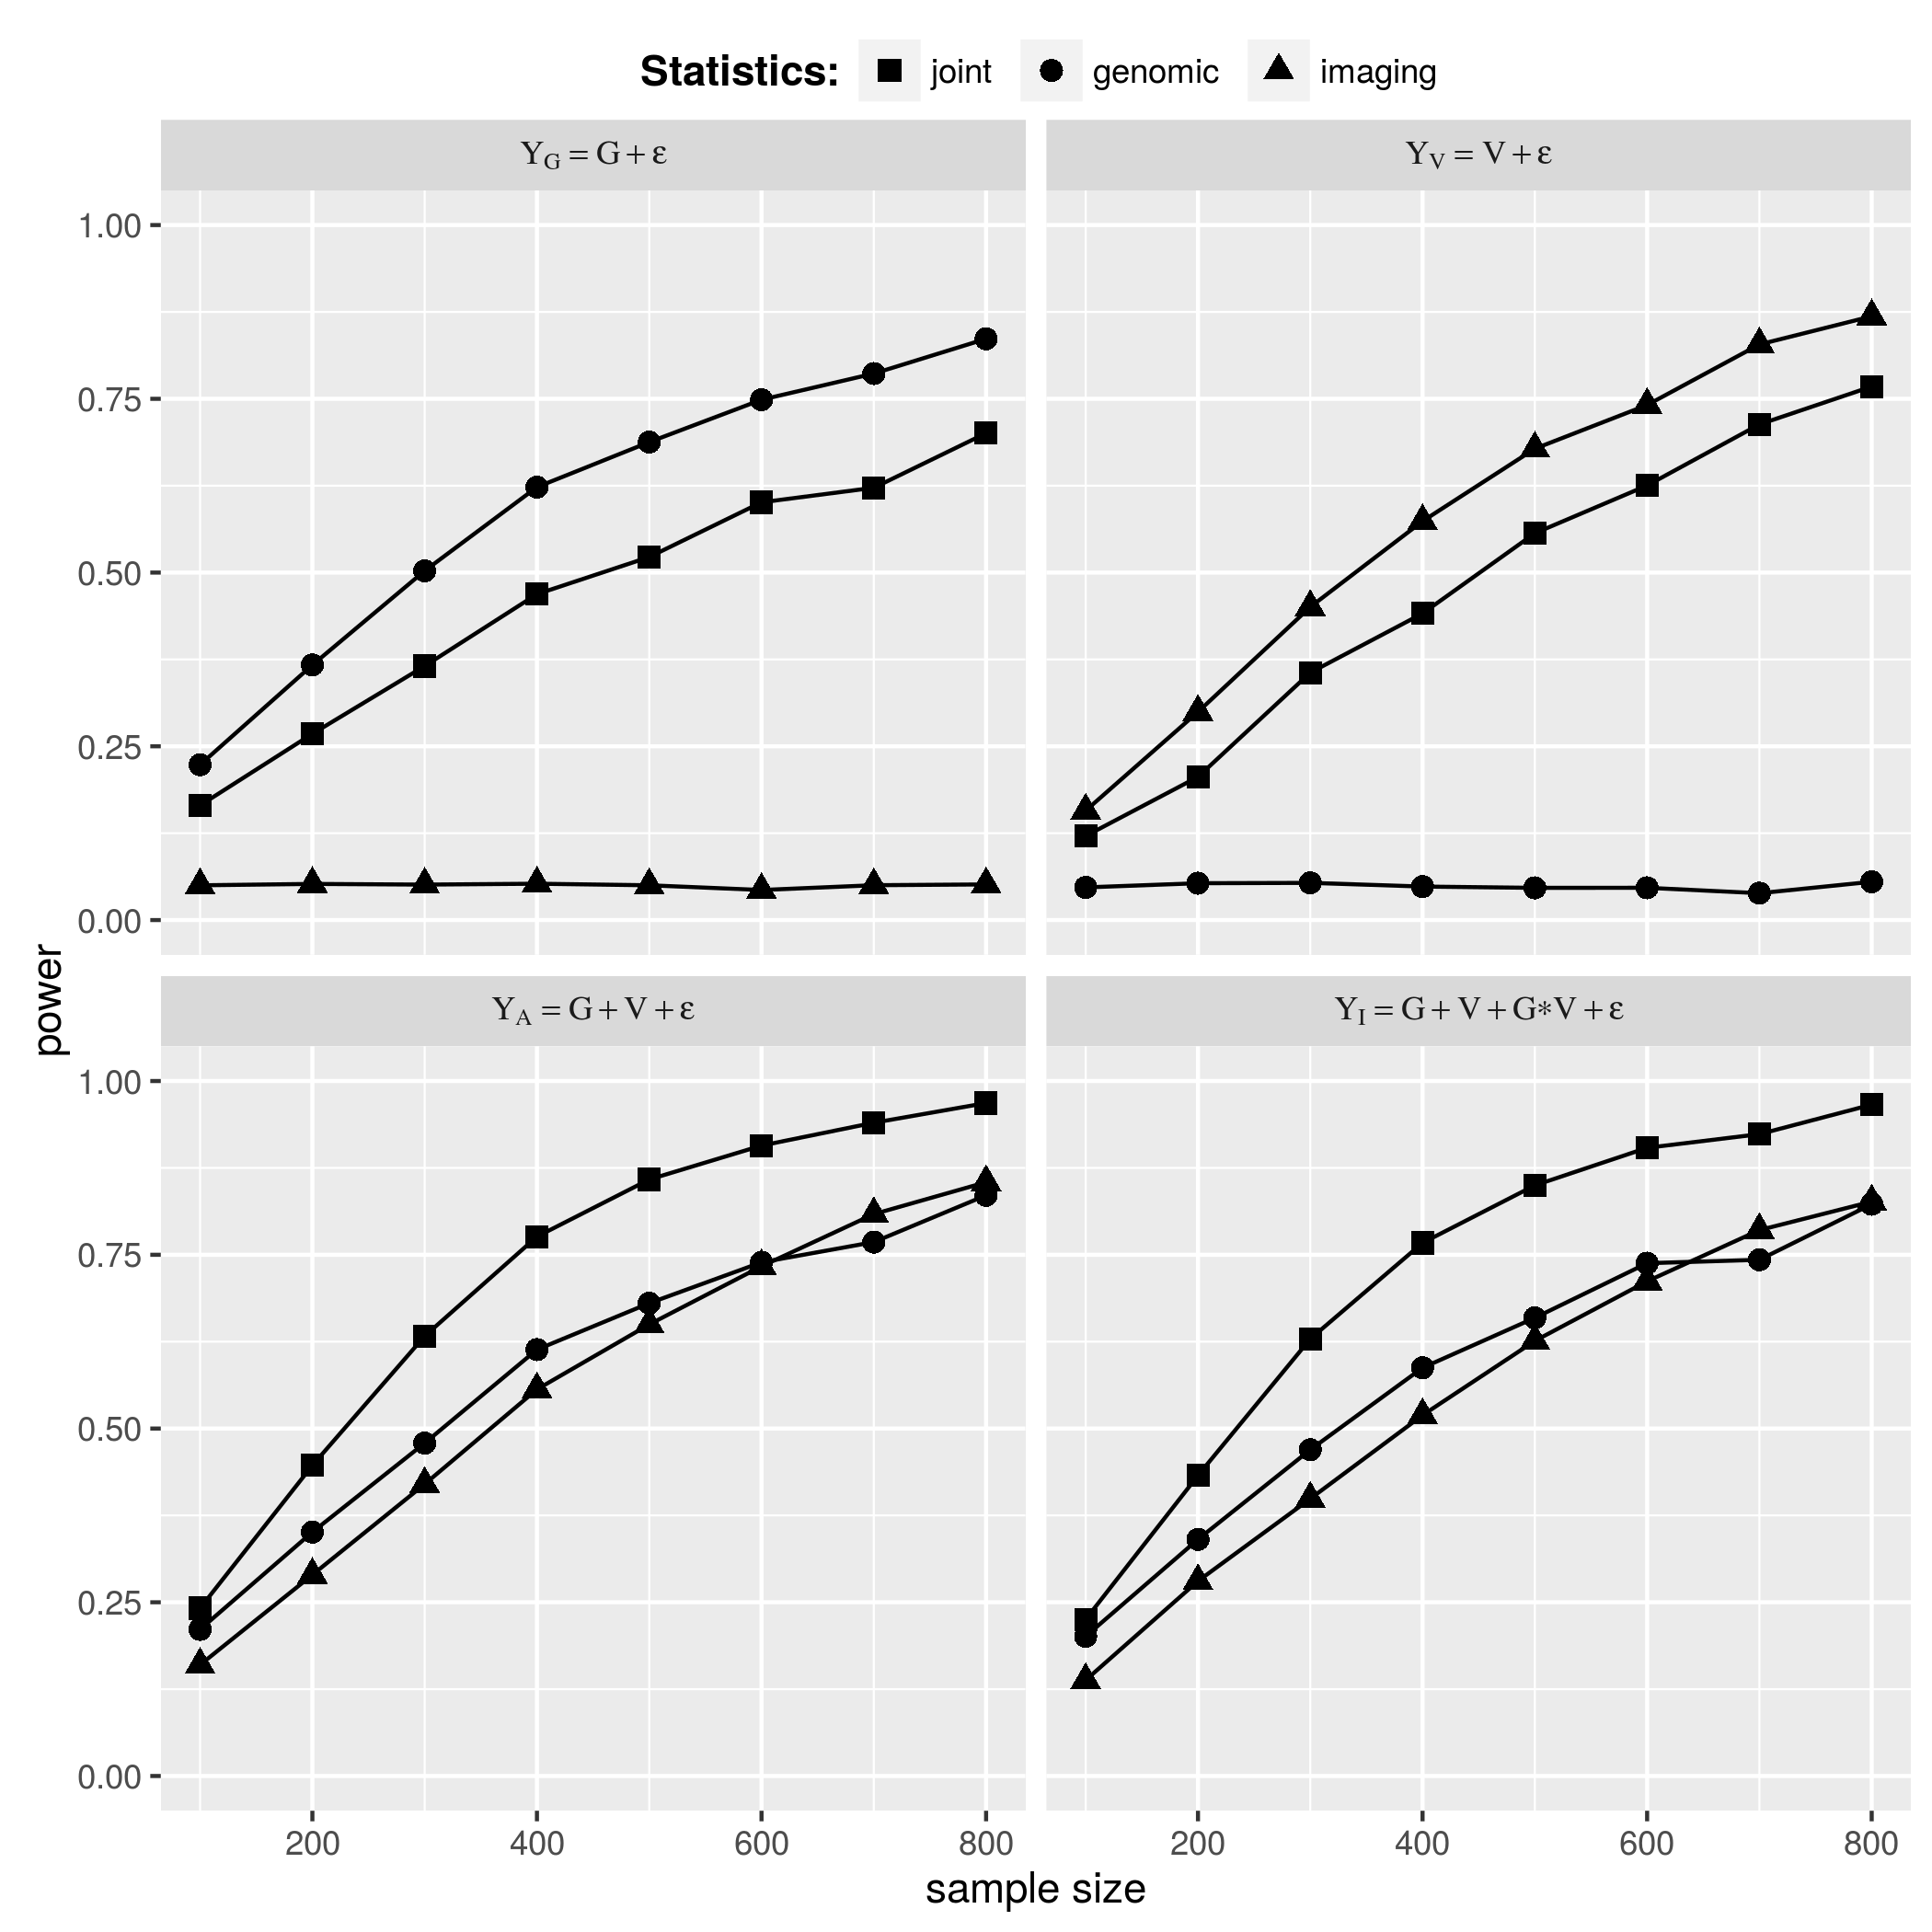
\includegraphics[width=300px]{img/PWR_CNT_KNL.png}
  \caption{Joint U v.s.\ genetic U and imaging U}\label{fig:PWR_CNT_KNL}
\end{figure} \\
The top row of Figure~\ref{fig:PWR_CNT_KNL} shows the two simpler statistics $U_G$ and $U_V$ performed best when they are indeed parsimonious, that is, the phenotypes were truly genomic or imaging based, but they are powerless when the phenotype does not concur the choice of kernels. In contrast, the joint statistic $U_J$ performed fairly well in both cases, closer to the correct parsimonious model, and the bottom row shows that $U_J$ outperformed other statistics when the phenotype involves both genomic and imaging effects.

\subsubsection{Grouping and Aggregation on Imaging}
Imaging variants do not suffer ``low MAF'' like rare genomic variants do, but grouping and aggregation technique may still be helpful by avoiding multiple testing of similar hypothesis. Under the same settings, we evaluate the performance of cortex regional analysis, versus false discovery rate (FDR) corrected VWA.\ Here we skipped the test of $H_0^G$, since the statistic $U_G$ does not rely on imaging profile. The result is shown in Figure~\ref{fig:PWR_CNT_VWA}.
\begin{figure}[!htbp]
  \centering
  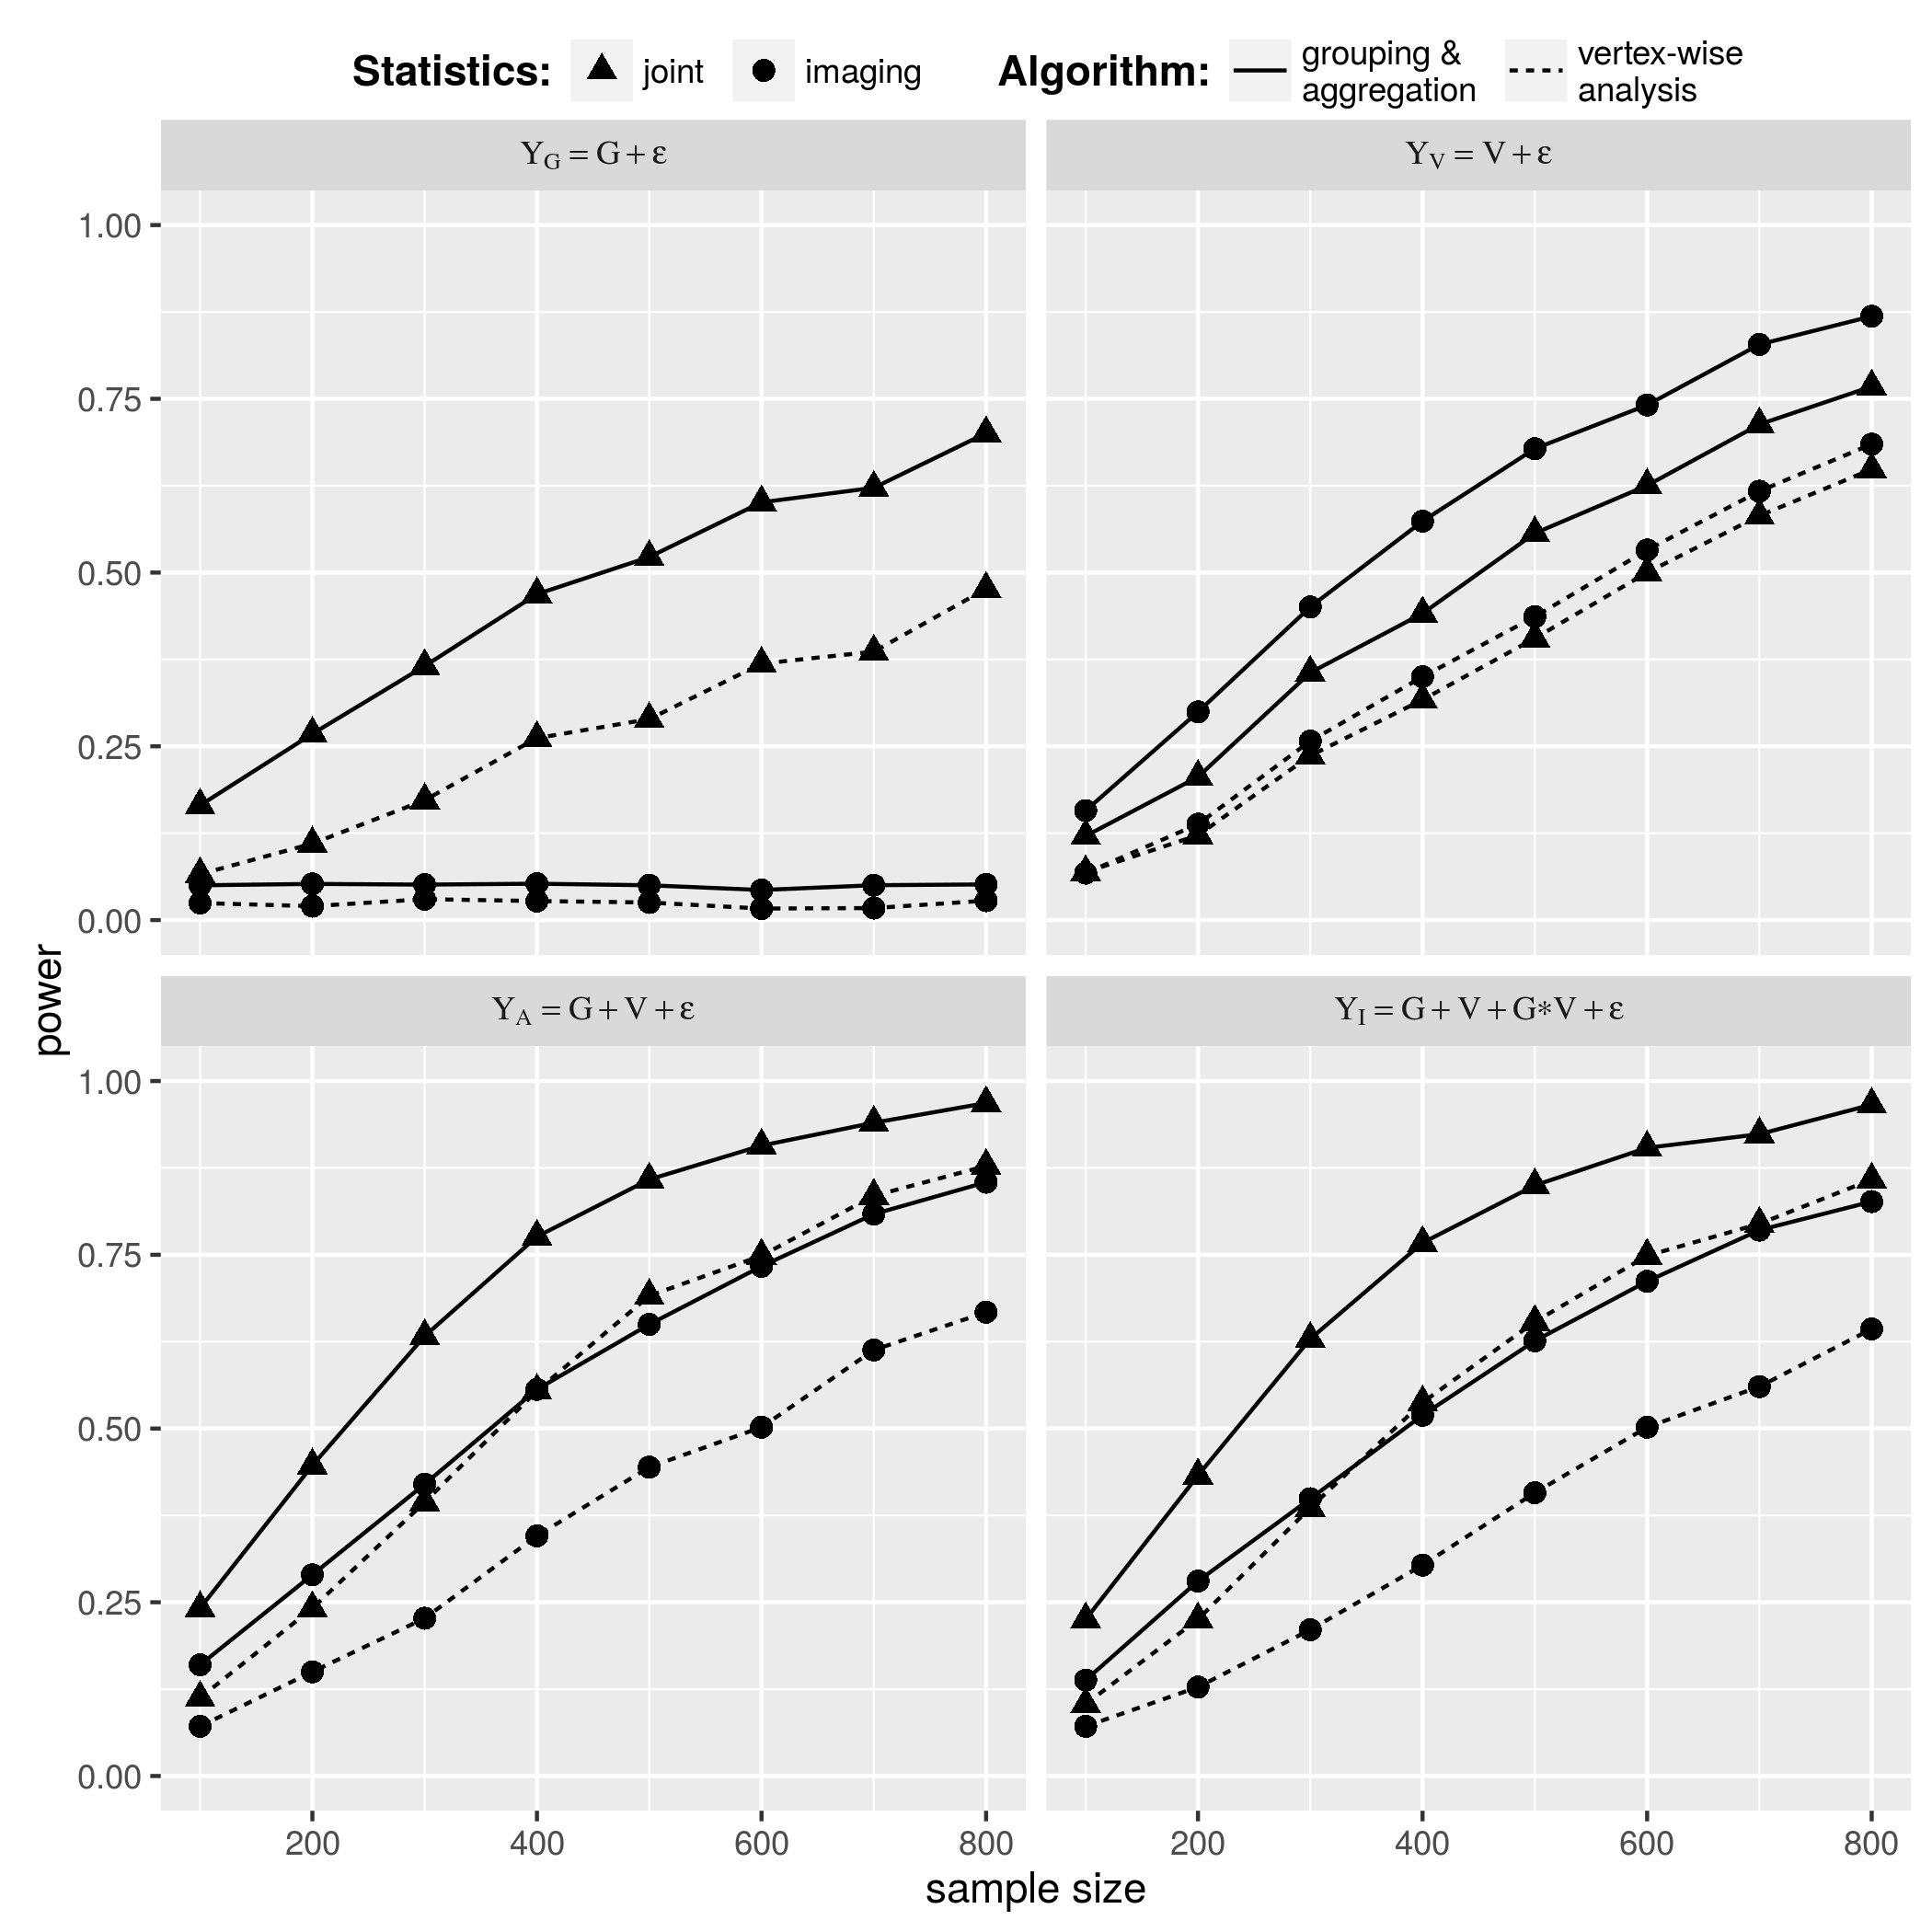
\includegraphics[width=300px]{img/PWR_CNT_VWA.png}
  \caption{Grouping \& Aggregation v.s.\ Vertex-wise Analysis}\label{fig:PWR_CNT_VWA}
\end{figure}
The aggregated test (solid lines) overpowers VWA (dashed lines) by large margins in all scenarios. An interesting speculation is when the kernels are completely misspecified, the type I error rate of VWA is below 0.05 (Figure~\ref{fig:PWR_CNT_VWA}, top left panel), which means the tests of each vertex (512 of them) are correlated, and caused FDR correction to be conservative. 

\subsubsection{High Order Imaging Features}
In this set of simulations we compare the use of high order features versus raw imaging profiles. The result is shown in Figure~\ref{fig:PWR_CNT_SAE} (again opt out testing $H_0^G$).
\begin{figure}[!htbp]
  \centering
  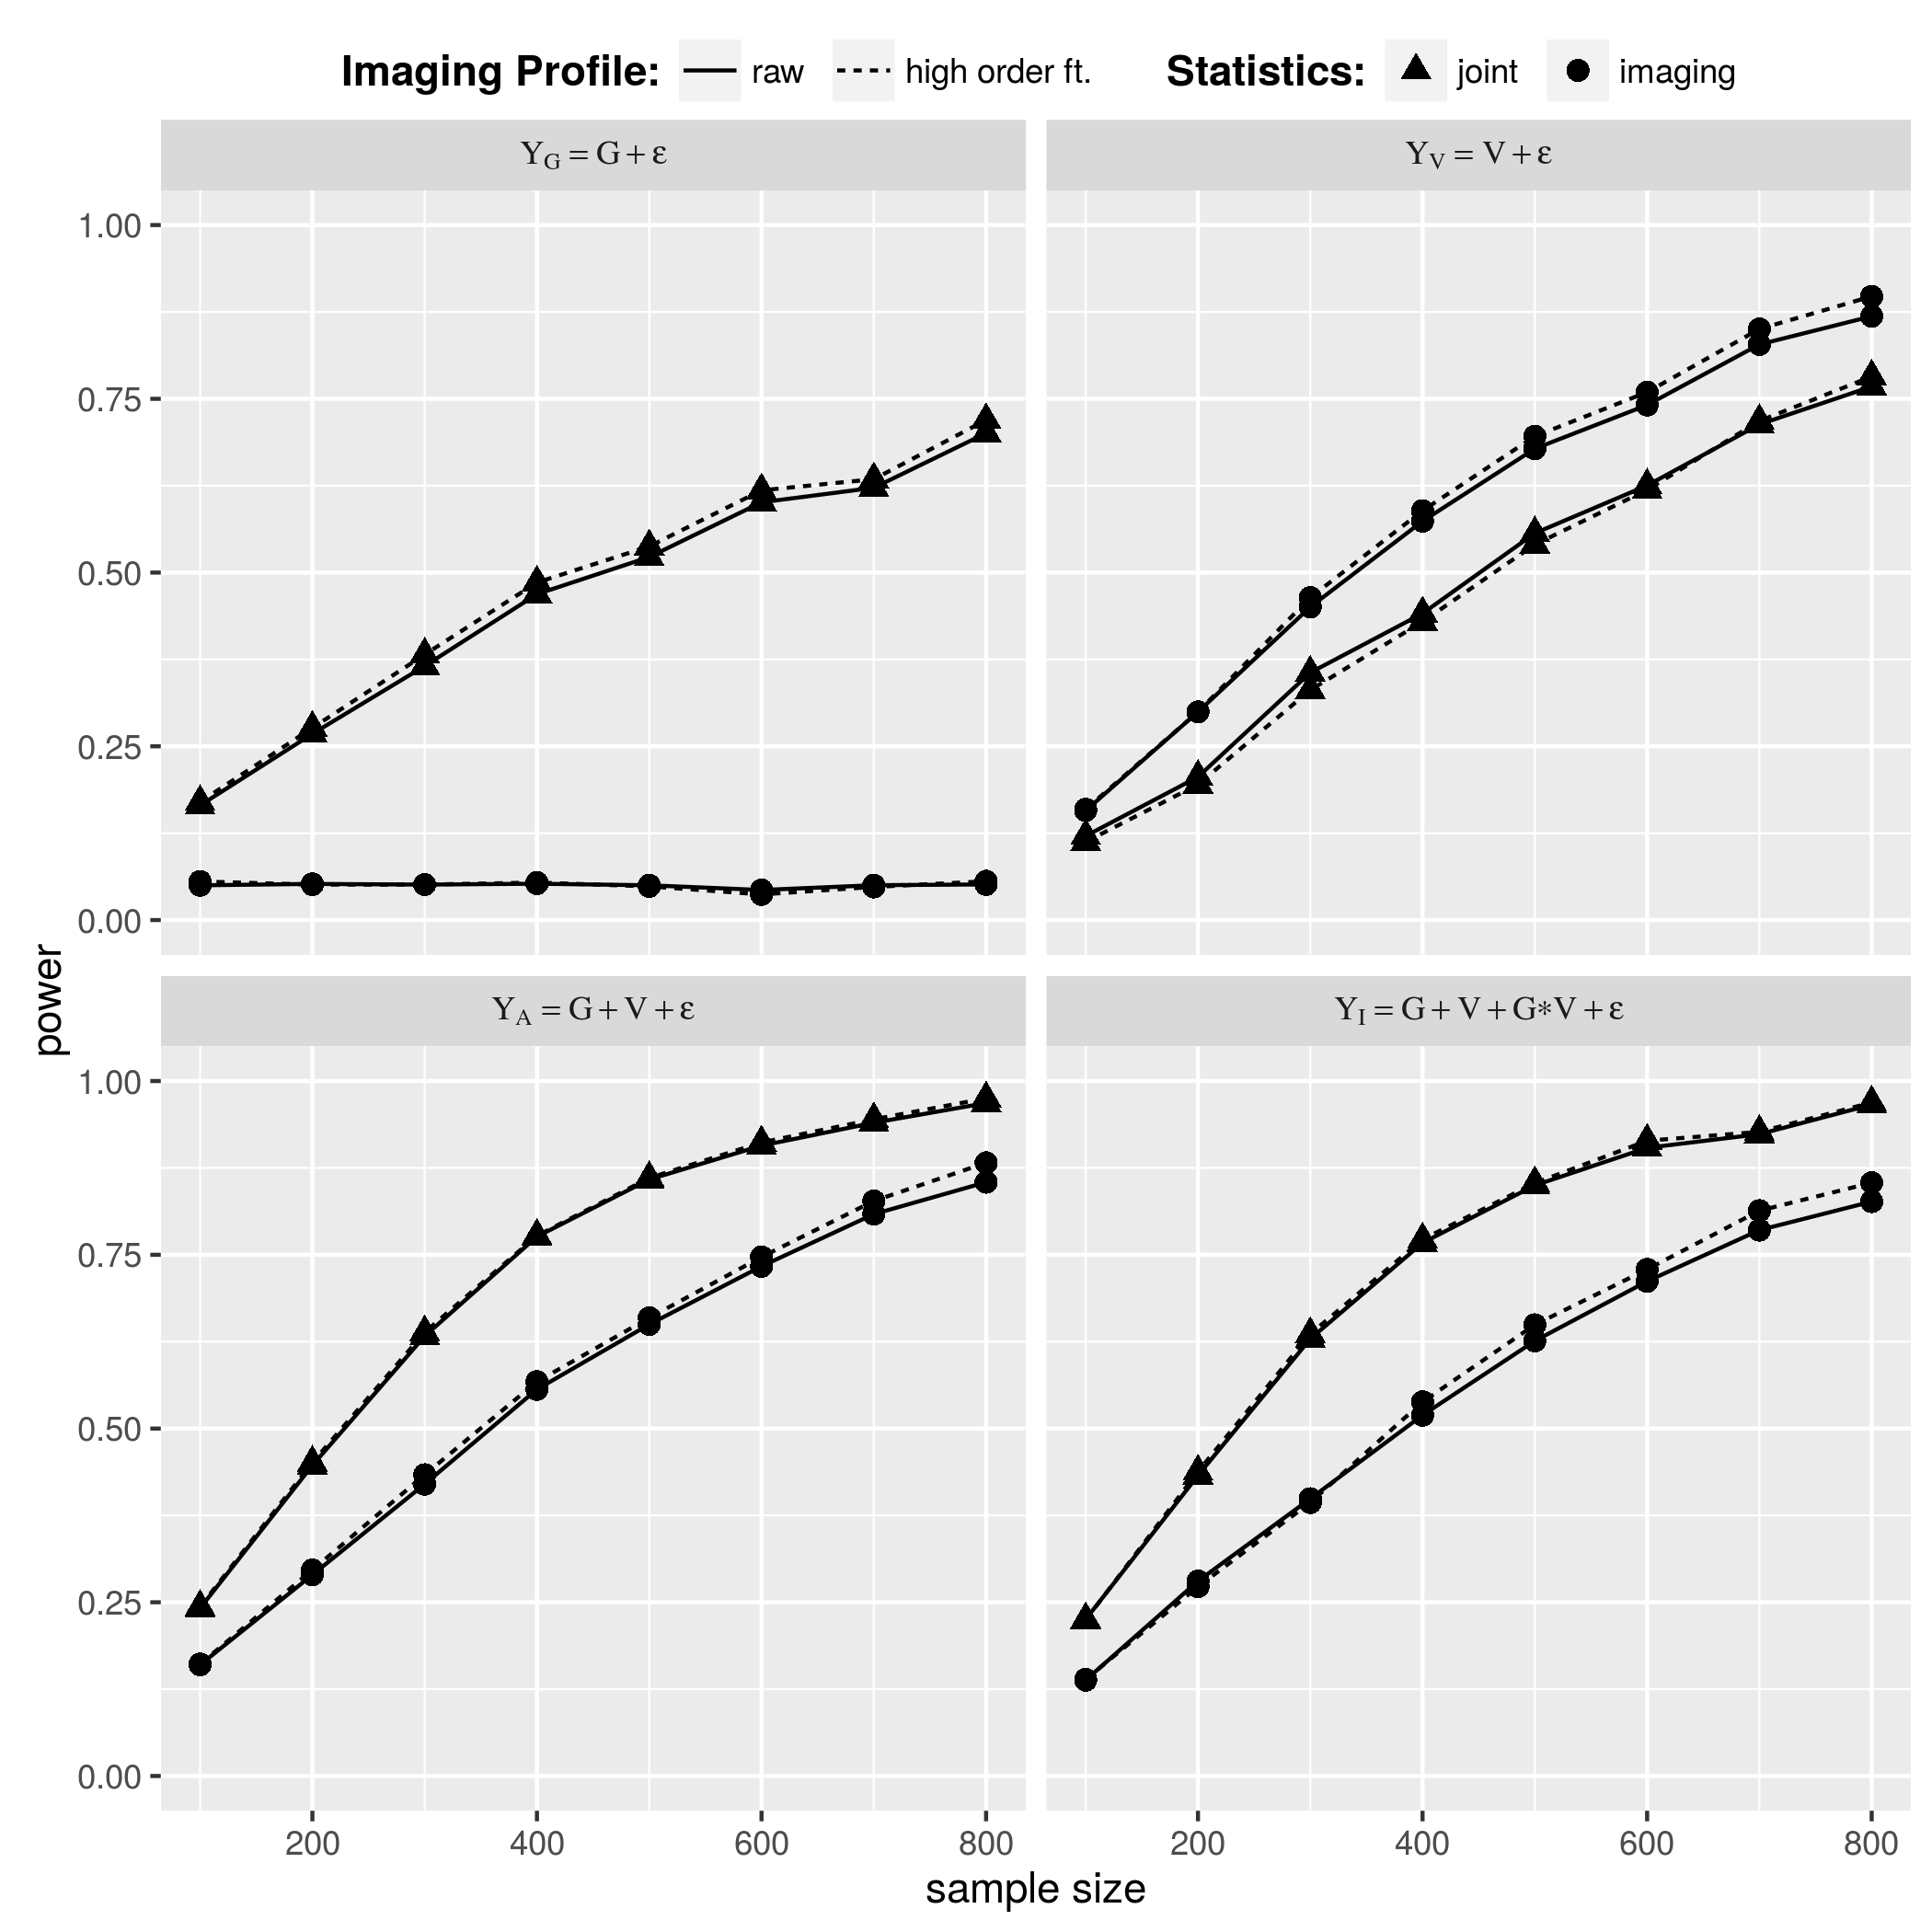
\includegraphics[width=300px]{img/PWR_CNT_SAE.png}
  \caption{High Order Features v.s.\ Original Vertices}\label{fig:PWR_CNT_SAE}
\end{figure}
Except the combination of lower sample size and the joint U statistic being partially redundant (Figure~\ref{fig:PWR_CNT_SAE}, top right), replacing raw imaging profile (Figure~\ref{fig:PWR_CNT_SAE}, solid lines) with their high order features (Figure~\ref{fig:PWR_CNT_SAE}, dashed lines) results in slight gain of power. The top left panel in~\ref{fig:PWR_CNT_SAE} also reassured that using high order features does not deviate the type I error rate away from expected $0.05$.

\subsubsection{Binary Phenotypes}
Dichotomous phenotypes are generated by sending the aforementioned four continuous ones to the inverse logit function, then draw the case/control status from the resulting probabilities. In every scenario, the power performance shares very similar pattern to the continuous phenotype, which is presented in the appendix.

\subsection{Real Data Analysis}
The baseline data of 327 out of 806 participants having definite diagnosis of Alzheimer's Disease (AD) entered the analysis, among whom 47 are cases and the rest 280 are healthy controls. The genomic testing units are $40,039$ gene regions. The imaging testing units are the high order features of 68 cortical regions abstracted from the raw imaging using 68 SAs trained with all 806 samples. We first regressed the the case/control status on 7 risk factors of AD, namely age, gender, race, ethnicity, years of education, marriage status, ever smoking, and APOE $\epsilon4$ haplotype, then the residuals are taken as phenotype to construct the U statistics. In total, there are $40,039 \times 68 = 2,722,652$ combinations to test the joint U statistic $U_J$, also for the purpose of comparison, we tested the two simplified $U_G$ and $U_V$, as a result, triplets of negative log transformed p-values $(P_J, P_G, P_V)$ for each combination are horizontally laid out in Figure~\ref{fig:RDA_PVL}, ordered by ascending $P_J$.
\begin{figure}[!htbp]
  \centering
  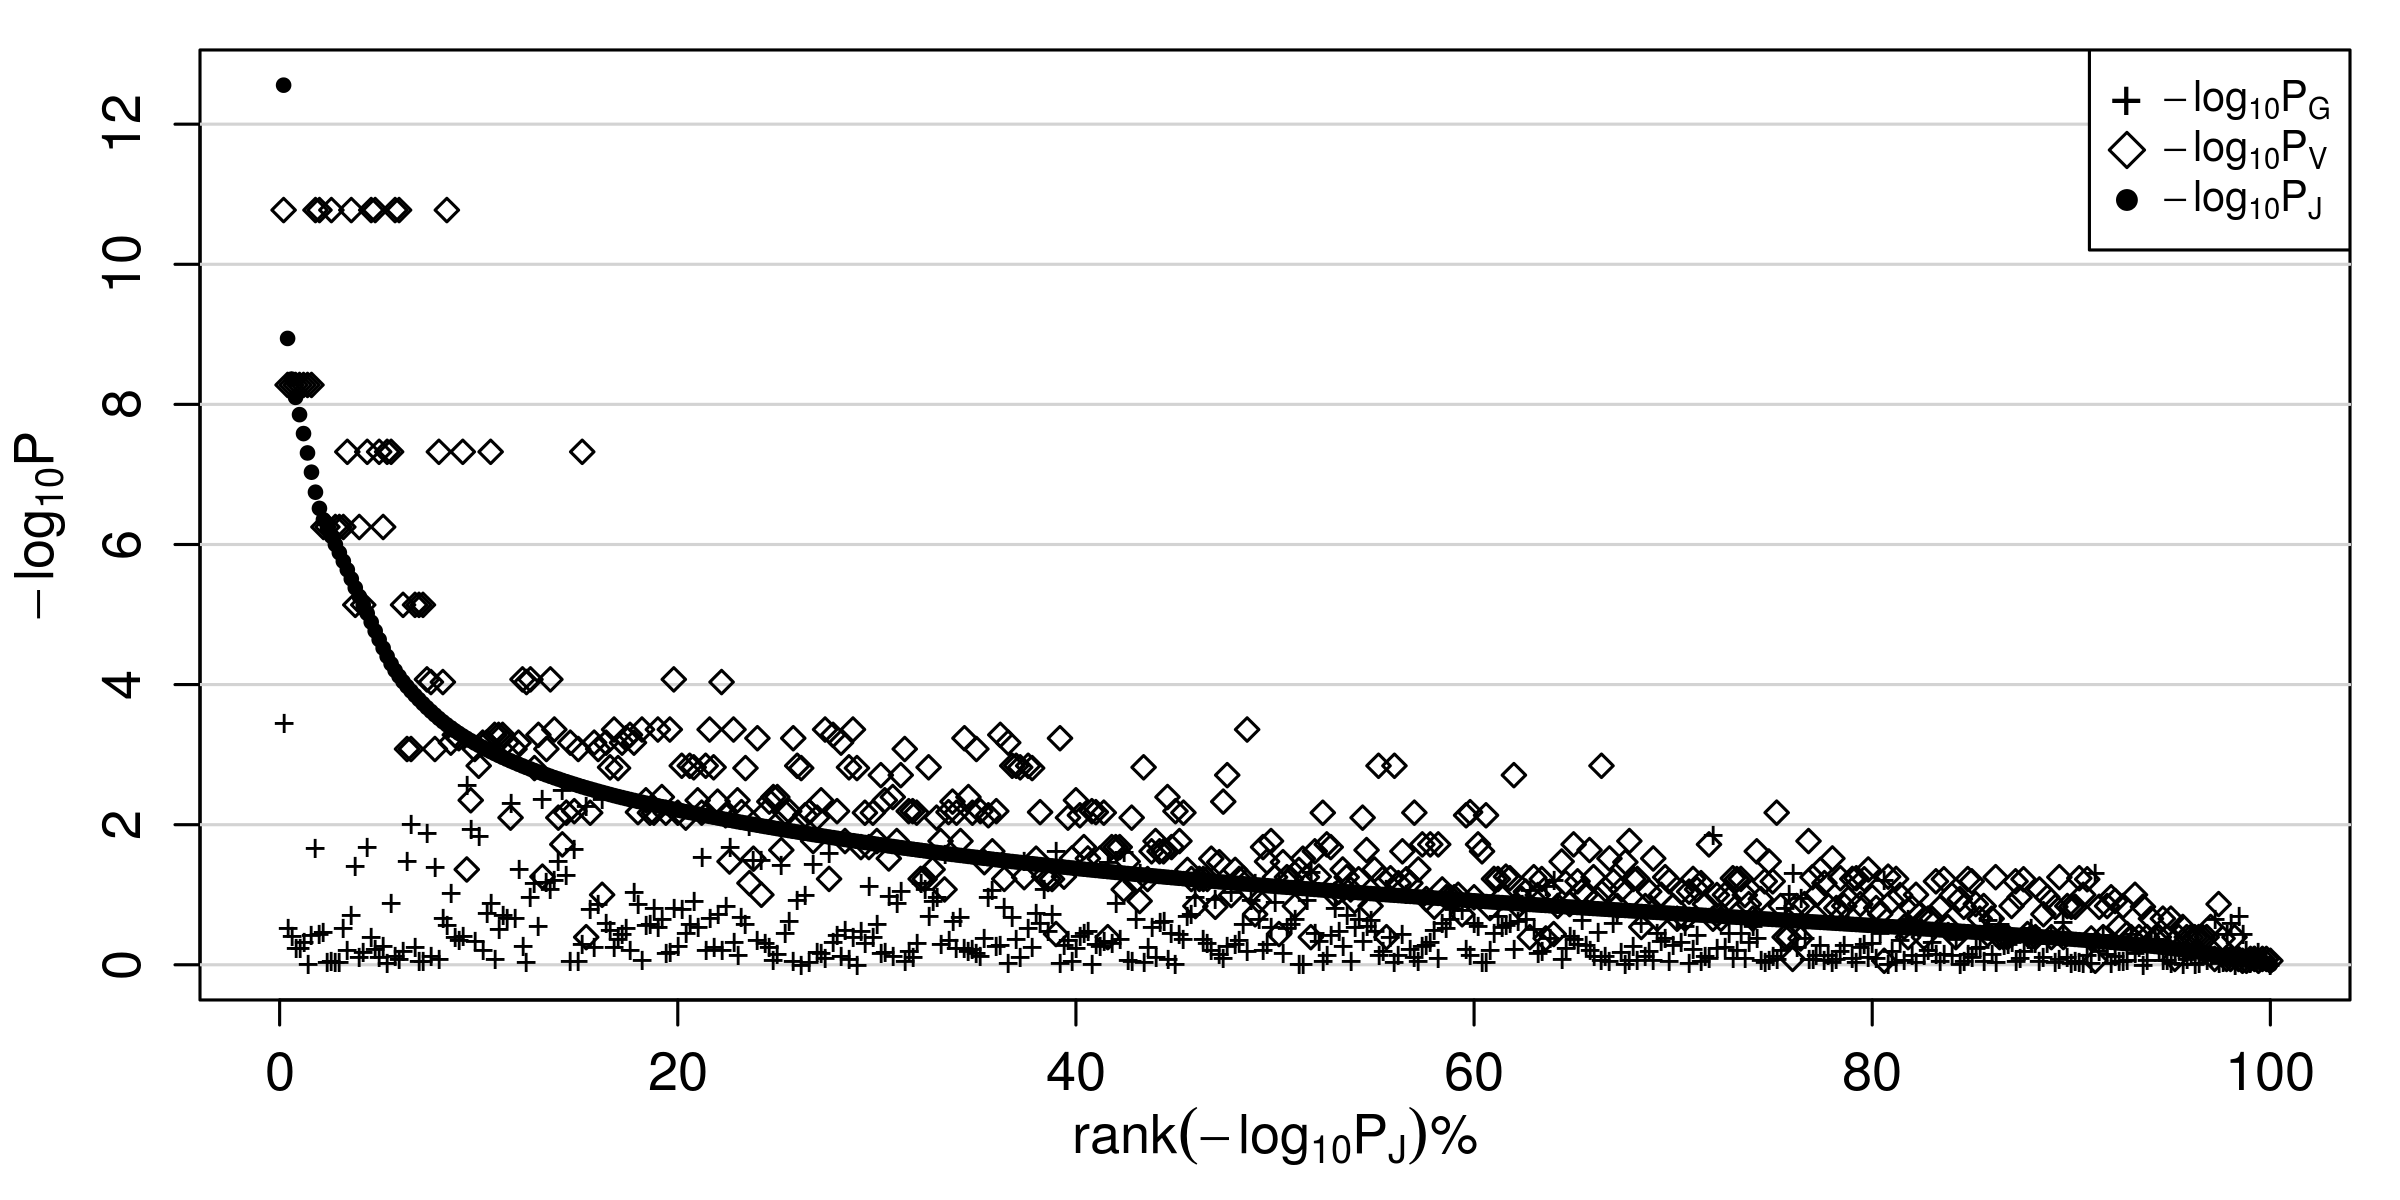
\includegraphics[width=300px]{img/RDA_PVL.png}
  \caption{p-values of real data analysis}\label{fig:RDA_PVL}
\end{figure}
The genomic based $U_G$ statistic by itself (Figure~\ref{fig:RDA_PVL}, crosses) never reached statistical significance after FDR correction of $40,039$ tests. The signal of imaging based $U_V$ (Figure~\ref{fig:RDA_PVL}, diamonds) in general is stronger than the genomic based $U_G$, reflecting the fact that upstream genomic effect is rather weak compared with the downstream cortex structure which is a strong indicator of neurological disorder. The significance of joint test $U_J$ (Figure~\ref{fig:RDA_PVL}, dots) lies between the two, leaning closer to the imaging based $U_V$. Notice that how $U_J$ ``borrows'' information from the imaging profile to enhance the signal of genomic based $U_G$, that is, when both $U_G$ and $U_V$ in the triplet are moderately significant, the joint statistic $U_J$ is likely to be more significant than either $U_G$ and $U_V$ alone, reaching the 0.05 threshold even after FDR correction of $2,680,894$ tests, which is demonstrate by the dots in the top left section of Figure~\ref{fig:RDA_PVL}, and corresponds to the 20 most significant triplets listed in Table~\ref{tab:RDA_T20}.
\begin{table}[!htbp]
  \centering
  \small
  \caption{Top 20 most significant joint test, overall}\label{tab:RDA_T20}
  % latex table generated in R 3.3.1 by xtable 1.8-0 package
% Fri Dec 23 17:55:43 2016
\begin{tabular}{llcclll}
  \hline
  GENE & CORTEX & $|V|$ & $|G|$ & $\qquad P_G$ & \qquad $P_V$ & \qquad $P_J$ \\ 
  \hline
  IGLV1-44 & l.superiortemporal & 7271 &  174 & $3.51 \times {10^{-04}}$ & $1.68 \times {10^{-11}}{_+^*}$ & $2.77 \times {10^{-13}}{_+^*}$ \\ 
  NBEAP2 & l.superiortemporal & 7271 &  238 & $1.19 \times {10^{-04}}$ & $1.68 \times {10^{-11}}{_+^*}$ & $4.74 \times {10^{-13}}{_+^*}$ \\ 
  RPL21P89 & l.superiortemporal & 7271 &   90 & $6.36 \times {10^{-04}}$ & $1.68 \times {10^{-11}}{_+^*}$ & $5.14 \times {10^{-13}}{_+^*}$ \\ 
  LOC102724504 & l.superiortemporal & 7271 &   59 & $1.41 \times {10^{-03}}$ & $1.68 \times {10^{-11}}{_+^*}$ & $5.56 \times {10^{-13}}{_+^*}$ \\ 
  CNTNAP3P8 & l.superiortemporal & 7271 &   40 & $1.08 \times {10^{-03}}$ & $1.68 \times {10^{-11}}{_+^*}$ & $6.17 \times {10^{-13}}{_+^*}$ \\ 
  CDH4 & l.superiortemporal & 7271 & 9464 & $4.64 \times {10^{-03}}$ & $1.68 \times {10^{-11}}{_+^*}$ & $6.96 \times {10^{-13}}{_+^*}$ \\ 
  HNRNPA1P19 & l.superiortemporal & 7271 &   17 & $8.88 \times {10^{-04}}$ & $1.68 \times {10^{-11}}{_+^*}$ & $7.80 \times {10^{-13}}{_+^*}$ \\ 
  FAM72C & l.superiortemporal & 7271 &  174 & $9.28 \times {10^{-06}}$ & $1.68 \times {10^{-11}}{_+^*}$ & $7.82 \times {10^{-13}}{_+^*}$ \\ 
  RP11-638L3.1 & l.superiortemporal & 7271 & 4067 & $1.41 \times {10^{-1}}$ & $1.68 \times {10^{-11}}{_+^*}$ & $9.49 \times {10^{-13}}{_+^*}$ \\ 
  CPXM1 & l.superiortemporal & 7271 &  208 & $8.78 \times {10^{-4}}$ & $1.68 \times {10^{-11}}{_+^*}$ & $1.08 \times {10^{-12}}{_+^*}$ \\ 
  LOC101929612 & l.superiortemporal & 7271 &  256 & $1.44 \times {10^{-2}}$ & $1.68 \times {10^{-11}}{_+^*}$ & $1.15 \times {10^{-12}}{_+^*}$ \\ 
  LOC100996517 & l.superiortemporal & 7271 &   34 & $6.77 \times {10^{-4}}$ & $1.68 \times {10^{-11}}{_+^*}$ & $1.20 \times {10^{-12}}{_+^*}$ \\ 
  IGLV5-45 & l.superiortemporal & 7271 &  179 & $3.44 \times {10^{-4}}$ & $1.68 \times {10^{-11}}{_+^*}$ & $1.23 \times {10^{-12}}{_+^*}$ \\ 
  MIS18BP1 & l.superiortemporal & 7271 &  553 & $4.95 \times {10^{-3}}$ & $1.68 \times {10^{-11}}{_+^*}$ & $1.35 \times {10^{-12}}{_+^*}$ \\ 
  CDR2 & l.superiortemporal & 7271 &  260 & $1.82 \times {10^{-4}}$ & $1.68 \times {10^{-11}}{_+^*}$ & $1.39 \times {10^{-12}}{_+^*}$ \\ 
  RPL41P2 & l.superiortemporal & 7271 &   87 & $6.04 \times {10^{-3}}$ & $1.68 \times {10^{-11}}{_+^*}$ & $1.59 \times {10^{-12}}{_+^*}$ \\ 
  LOC101927737 & l.superiortemporal & 7271 &  157 & $7.20 \times {10^{-3}}$ & $1.68 \times {10^{-11}}{_+^*}$ & $1.60 \times {10^{-12}}{_+^*}$ \\ 
  IGLV1-47 & l.superiortemporal & 7271 &  138 & $1.44 \times {10^{-2}}$ & $1.68 \times {10^{-11}}{_+^*}$ & $1.60 \times {10^{-12}}{_+^*}$ \\ 
  IGLV7-46 & l.superiortemporal & 7271 &  130 & $9.15 \times {10^{-4}}$ & $1.68 \times {10^{-11}}{_+^*}$ & $1.69 \times {10^{-12}}{_+^*}$ \\ 
  ZDHHC15 & l.superiortemporal & 7271 &   80 & $1.56 \times {10^{-3}}$ & $1.68 \times {10^{-11}}{_+^*}$ & $1.73 \times {10^{-12}}{_+^*}$ \\ 
  \hline
  \multicolumn{7}{l}{\texttt{*: below 0.05 after Bonferroni correction}} \\ 

  \multicolumn{7}{l}{\texttt{+: below 0.01 after FDR correction}}        \\ \hline
\end{tabular}

\end{table} \\
From Table~\ref{tab:RDA_T20} we see the top 20 most significant test all involves left-superior-temporal, whose neuron loss and shrinkage is strongly associated with the onset of Alzheimer's Disease and its progression to dementia~\cite{AD:ST1}. 

To see more diverse cases of incorporating imaging profile to enhance signal of genomic analysis, we compiled the most significant $U_J$ involving each of the 68 regions and listed the top 20 in Table~\ref{tab:RDA_JNT}.
\begin{table}[!htbp]
  \centering
  \small
  \caption{top 20 most significant joint test, per cortex region}\label{tab:RDA_JNT}
  % latex table generated in R 3.3.1 by xtable 1.8-0 package
% Fri Dec 23 17:55:45 2016
\begin{tabular}{llcclll}
  \hline
GENE & CORTEX & $|V|$ & $|G|$ & $\qquad P_G$ & \qquad $P_V$ & \qquad $P_J$ \\ 
  \hline
IGLV1-44 & l.superiortemporal & 7271 &  174 & $3.51 \times {10^{-4}}$ & $1.68 \times {10^{-11}}{_+^*}$ & $2.77 \times {10^{-13}}{_+^*}$ \\ 
  ZNF749 & l.entorhinal & 1102 &  321 & $2.67 \times {10^{-5}}$ & $5.28 \times {10^{-9}}{_+^*}$ & $2.63 \times {10^{-11}}{_+^*}$ \\ 
  FAM72C & r.superiortemporal & 6868 &  174 & $9.28 \times {10^{-6}}$ & $4.75 \times {10^{-8}}{_+^*}$ & $2.14 \times {10^{-10}}{_+^*}$ \\ 
  ZNF749 & r.entorhinal &  902 &  321 & $2.67 \times {10^{-5}}$ & $5.62 \times {10^{-7}}{_+^*}$ & $1.08 \times {10^{-9}}{_+^*}$ \\ 
  FAM72C & l.cuneus & 1630 &  174 & $9.28 \times {10^{-6}}$ & $7.27 \times {10^{-6}}{_+^*}$ & $4.22 \times {10^{-9}}{_+^*}$ \\ 
  ZNF749 & l.fusiform & 4714 &  321 & $2.67 \times {10^{-5}}$ & $8.43 \times {10^{-5}}{_+^*}$ & $4.54 \times {10^{-8}}{_+}$ \\ 
  FAM72C & l.middletemporal & 4452 &  174 & $9.28 \times {10^{-6}}$ & $4.38 \times {10^{-4}}{_+^*}$ & $5.14 \times {10^{-8}}{_+}$ \\ 
  FAM72C & r.cuneus & 1638 &  174 & $9.28 \times {10^{-6}}$ & $8.31 \times {10^{-4}}{_+}$ & $6.33 \times {10^{-8}}{_+}$ \\ 
  ZNF749 & l.temporalpole &  839 &  321 & $2.67 \times {10^{-5}}$ & $9.20 \times {10^{-5}}{_+^*}$ & $7.05 \times {10^{-8}}{_+}$ \\ 
  FAM72C & r.precuneus & 7975 &  174 & $9.28 \times {10^{-6}}$ & $1.44 \times {10^{-3}}{_+}$ & $7.43 \times {10^{-8}}{_+}$ \\ 
  HSPD1P13 & l.pericalcarine & 1912 &   86 & $1.69 \times {10^{-5}}$ & $6.74 \times {10^{-4}}{_+^*}$ & $1.12 \times {10^{-7}}{_+}$ \\ 
  FAM72C & r.fusiform & 4661 &  174 & $9.28 \times {10^{-6}}$ & $5.83 \times {10^{-4}}{_+^*}$ & $1.18 \times {10^{-7}}{_+}$ \\ 
  HSPD1P13 & r.pericalcarine & 1823 &   86 & $1.69 \times {10^{-5}}$ & $5.22 \times {10^{-4}}{_+^*}$ & $1.50 \times {10^{-7}}{_+}$ \\ 
  FAM72C & r.precentral & 10705 &  174 & $9.28 \times {10^{-6}}$ & $6.73 \times {10^{-3}}$ & $2.15 \times {10^{-7}}{_+}$ \\ 
  HSPD1P13 & r.paracentral & 3831 &   86 & $1.69 \times {10^{-5}}$ & $1.91 \times {10^{-2}}$ & $2.41 \times {10^{-7}}{_+}$ \\ 
  ZNF749 & r.temporalpole &  817 &  321 & $2.67 \times {10^{-5}}$ & $1.55 \times {10^{-3}}{_+}$ & $3.30 \times {10^{-7}}{_+}$ \\ 
  FAM72C & l.precentral & 10740 &  174 & $9.28 \times {10^{-6}}$ & $6.62 \times {10^{-3}}$ & $3.94 \times {10^{-7}}{_+}$ \\ 
  FAM72C & l.superiorfrontal & 12179 &  174 & $9.28 \times {10^{-6}}$ & $1.96 \times {10^{-3}}{_+}$ & $4.39 \times {10^{-7}}{_+}$ \\ 
  FAM72C & l.postcentral & 9519 &  174 & $9.28 \times {10^{-6}}$ & $1.71 \times {10^{-2}}$ & $5.69 \times {10^{-7}}{_+}$ \\ 
  ZNF749 & l.insula & 5229 &  321 & $2.67 \times {10^{-5}}$ & $1.52 \times {10^{-3}}{_+}$ & $6.69 \times {10^{-7}}{_+}$ \\ 
   \hline
    \multicolumn{7}{l}{\texttt{*: below 0.05 after Bonferroni correction}} \\ 

    \multicolumn{7}{l}{\texttt{+: below 0.01 after FDR correction}}        \\ \hline
\end{tabular}

\end{table} \\
We see in some cases both the genomic and imaging based $U_G$ and $U_V$ do not reach statistical significance after multiple testing adjustment yet the joint statistic $U_J$ does, even if the number of combinations ($2,680,894$) is way larger than the number of genes ($40,039$) or cortex regions ($68$). These result suggest the existence of strong interaction, possibly mediation effect between the gene and cortex region.
